%%\documentclass[12pt,a4paper,titlepage]{article}
%%\usepackage[utf8]{inputenc}
%%\usepackage[russian]{babel}
%%\usepackage[OT1]{fontenc}
%%\usepackage{amsmath}
%%\usepackage{amsfonts}
%%\usepackage{amssymb}
%%\usepackage{listings}
%%\usepackage{graphicx}
%%\author{Богданов Н.Е.}
%%\title{
%Отчет по лабораторной работе №  1\\
%%по предмету \\«Информационная безопасность»\\
%%	\textbf{
%%		\begin{large}
%%Программа для шифрования и подписи GPG
%%		\end{large}
%%	}
%%}
%%\begin{document}
%%\maketitle
%%\tableofcontents
\newpage
\section{Постановка задачи}
\begin{enumerate}
	\item Установить и настроить пакет GPG 2
	\item Создать набор ключей в Kleopatra
	\item Экспортировать свой ключ, импортировать ключ другого участника эксперимента
	\item Зашифровать файл и отправить другому человеку, расшифровать чужой файл
	\item Выполнить те же пункты, используя консольный интерфейс
\end{enumerate}
\section{Используемые инструменты}
\begin{itemize}
\item GnuPG (Kleopatra) Version 2.2.0
\item ОС windows 7 x64
\end{itemize}
\section{GnuPG}
GNU Privacy Guard (GnuPG, GPG) — свободная программа для шифрования информации и создания электронных цифровых подписей. Разработана как альтернатива PGP и выпущена под свободной лицензией GNU General Public License. GnuPG полностью совместима со стандартом IETF OpenPGP. Текущие версии GnuPG могут взаимодействовать с PGP и другими OpenPGP-совместимыми системами.

Шифрование PGP осуществляется последовательно хешированием, сжатием данных, шифрованием с симметричным ключом, и, наконец, шифрованием с открытым ключом, причём каждый этап может осуществляться одним из нескольких поддерживаемых алгоритмов. 

\newpage
\section{Ход работы}
\subsection{Использование GPG с помощью интерфейса Kleopatra}

Установим и запустим программу Kleopatra. Перед нами появится главное окно:

\begin{figure}[!ht]
	\centering
	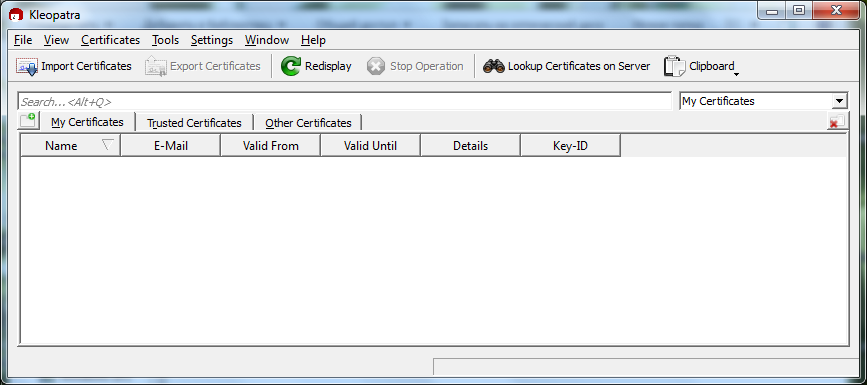
\includegraphics[width=0.5\textwidth]{images/1.png}
	\caption{Главное окно программы Kleopatra}
\end{figure}

Запустим мастер создания ключа. В данной работе нас интересуют ключи PGP.

\begin{figure}[!ht]
	\centering
	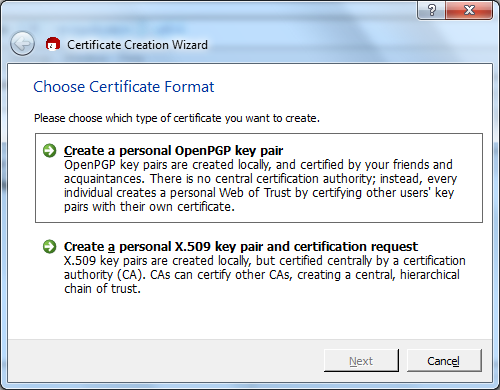
\includegraphics[width=0.7\textwidth]{images/2.png}
	\caption{Мастер создания ключа}
\end{figure}

Пользователь PGP создаёт ключевую пару: открытый и закрытый ключ. При генерации ключей задаются их владелец (имя и адрес электронной почты), тип ключа, длина ключа и срок его действия. 
Открытый ключ используется для шифрования и проверки цифровой подписи. Закрытый ключ — для декодирования и создания цифровой подписи.

\begin{figure}[!ht]
	\centering
	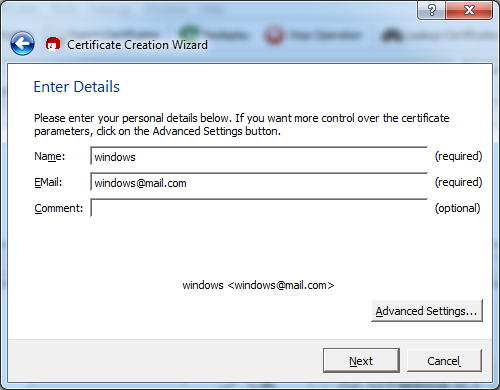
\includegraphics[width=0.5\textwidth]{images/3.png}
	\caption{Задание владельца ключа}
\end{figure}

PGP поддерживает три типа ключей RSA v4, RSA legacy (v3) и Diffie-Hellman/DSS (Elgamal в терминологии GnuPG).

\begin{figure}[!ht]
	\centering
	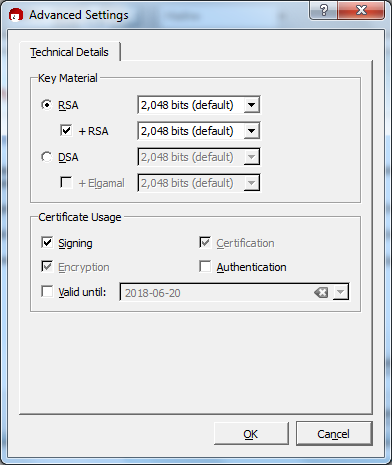
\includegraphics[width=0.5\textwidth]{images/4.png}
	\caption{Задание длинны и типа шифрования}
\end{figure}

Для ключей RSA legacy длина ключа может составлять от 1024 до 2048 бит, а для Diffie-Hellman/DSS и RSA — от 1024 до 4096. Ключи RSA legacy содержат одну ключевую пару, а ключи Diffie-Hellman/DSS и RSA могут содержать один главный ключ и дополнительные ключи для шифрования. При этом ключ электронной подписи в ключах Diffie-Hellman/DSS всегда имеет размер 1024. Срок действия для каждого из типов ключей может быть определён как неограниченный или до конкретной даты. Для защиты ключевого контейнера используется секретная фраза.

\begin{figure}[!ht]
	\centering
	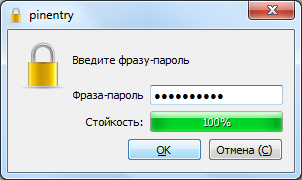
\includegraphics[width=0.3\textwidth]{images/5.png}
	\caption{Задание секретной фразы}
\end{figure}


\begin{figure}[!ht]
	\centering
	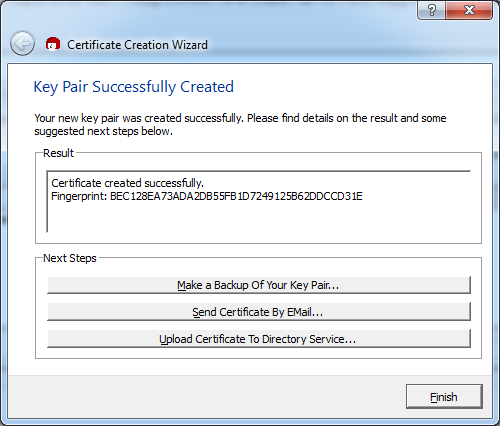
\includegraphics[width=0.5\textwidth]{images/6.png}
	\caption{Завершение создания ключа}
\end{figure}


\begin{figure}[!ht]
	\centering
	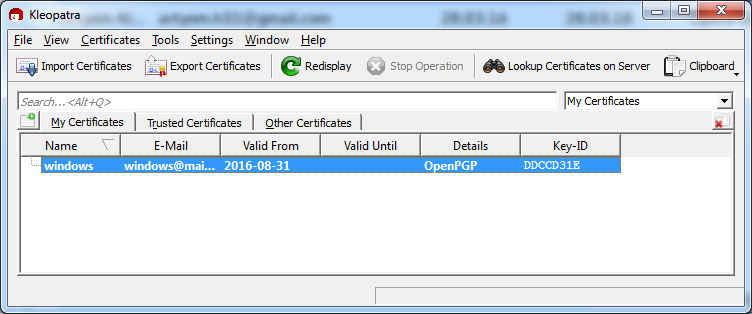
\includegraphics[width=0.7\textwidth]{images/7.png}
	\caption{Создание ключа}
\end{figure}

\newpage
Наш ключ появился в списке
Получим сертификат с другого компьютера
\begin{figure}[!ht]
	\centering
	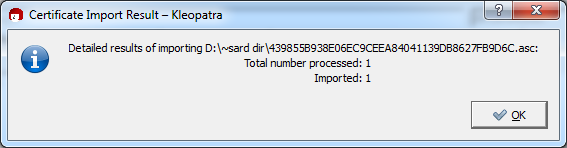
\includegraphics[width=0.5\textwidth]{images/8.png}
	\caption{Импорт сертификата}
\end{figure}

\begin{figure}[!ht]
	\centering
	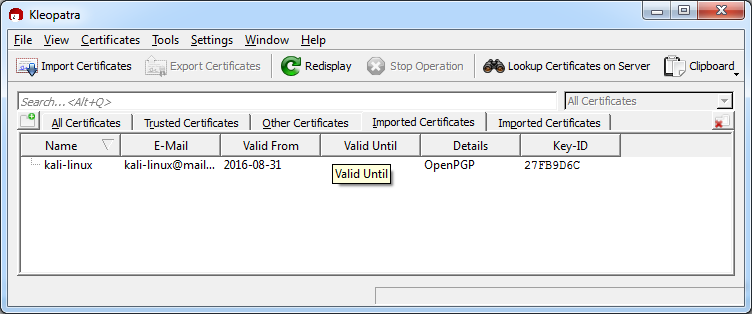
\includegraphics[width=0.5\textwidth]{images/9.png}
	\caption{Сертификаты}
\end{figure}

\begin{figure}[!ht]
	\centering
	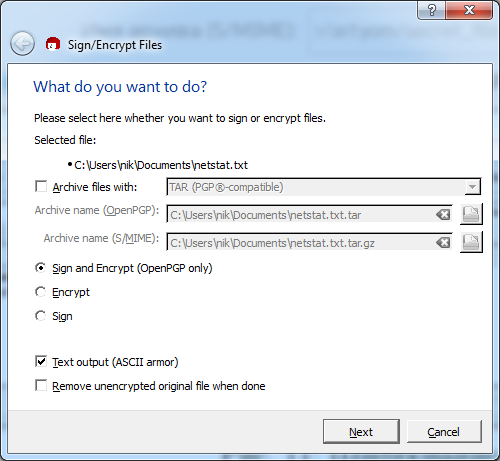
\includegraphics[width=0.5\textwidth]{images/10.png}
	\caption{Выбор файла для шифрования}
\end{figure}
\newpage
Выберем свой и чужой ключ
\begin{figure}[!ht]
	\centering
	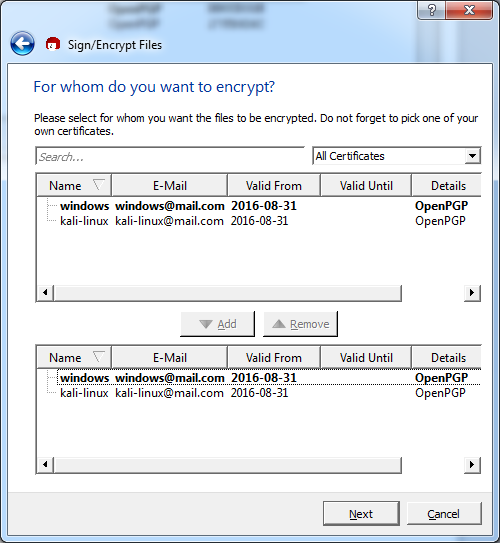
\includegraphics[width=0.5\textwidth]{images/11.png}
	\caption{Шифрование}
\end{figure}
\newpage
Выберем открытый ключ с помощью которого будем шифровать
\begin{figure}[!ht]
	\centering
	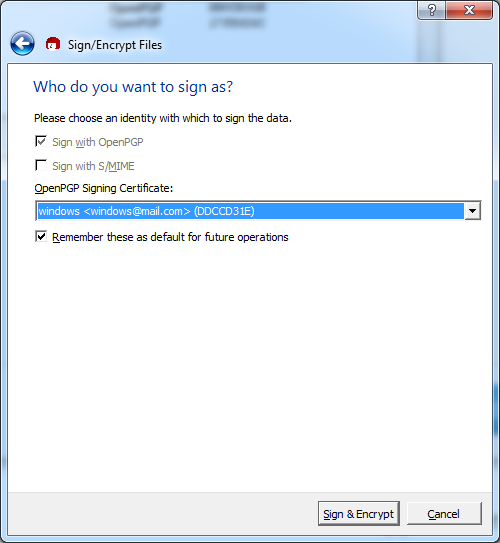
\includegraphics[width=0.5\textwidth]{images/12.png}
	\caption{Шифрование}
\end{figure}

Сообщение об успехе
\begin{figure}[!ht]
	\centering
	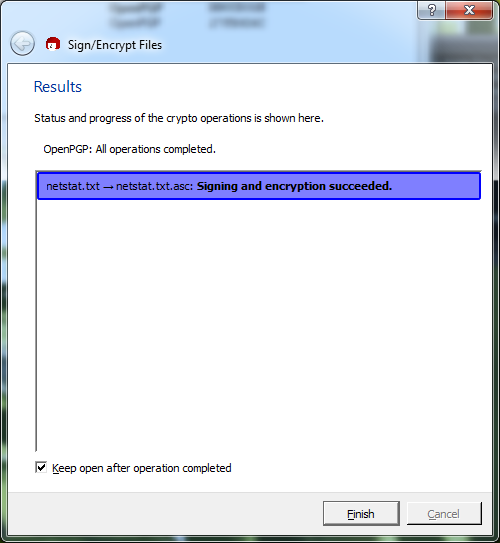
\includegraphics[width=0.5\textwidth]{images/13.png}
	\caption{Шифрование}
\end{figure}

Так выглядит зашифрованный файл
\begin{figure}[!ht]
	\centering
	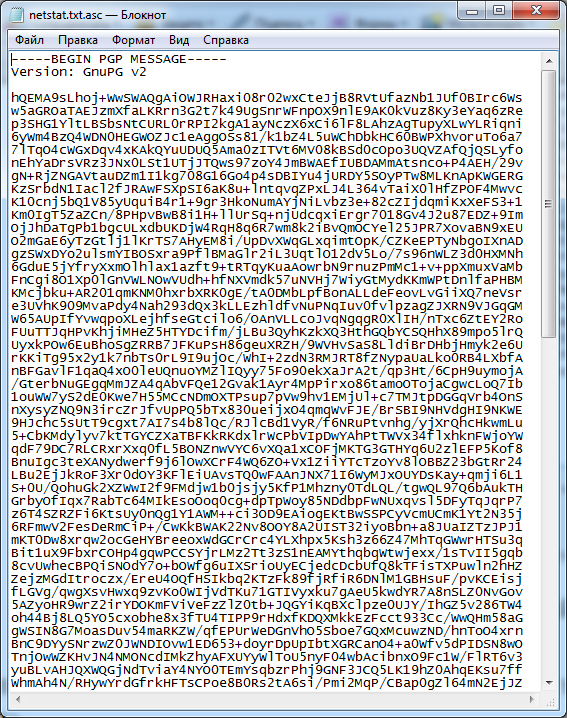
\includegraphics[width=0.5\textwidth]{images/14.png}
	\caption{Зашифрованный файл}
\end{figure}
\newpage
Теперь расшифруем файл
\begin{figure}[!ht]
	\centering
	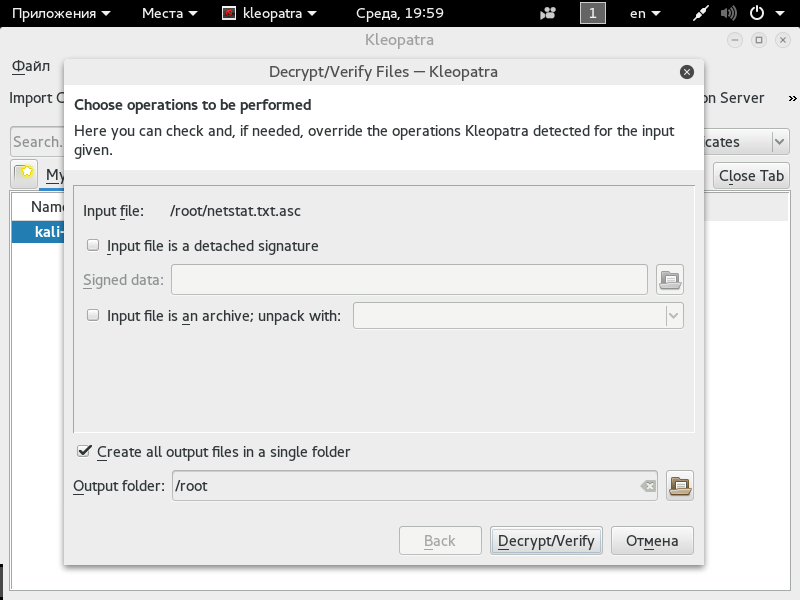
\includegraphics[width=0.6\textwidth]{images/16.png}
	\caption{Расшифровка}
\end{figure}
\begin{figure}[!ht]
	\centering
	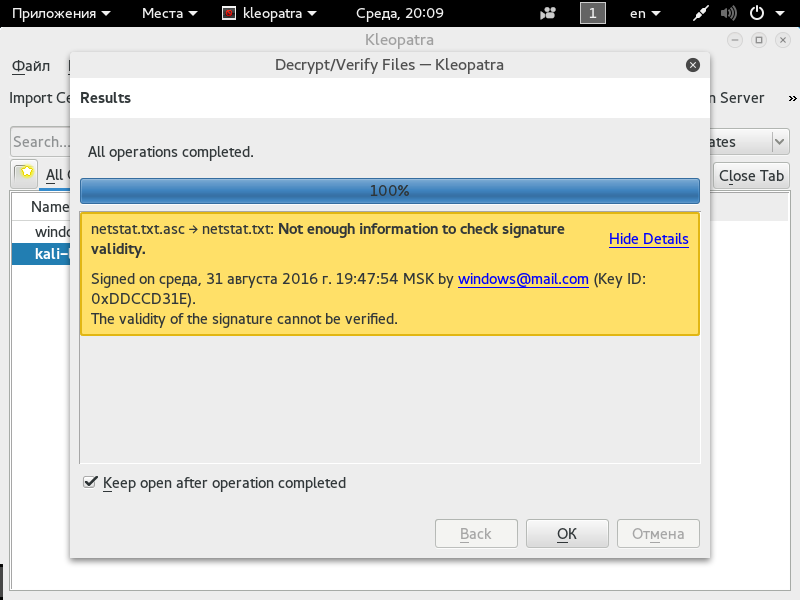
\includegraphics[width=0.6\textwidth]{images/17.png}
	\caption{Расшифровка}
\end{figure}
\begin{figure}[!ht]
	\centering
	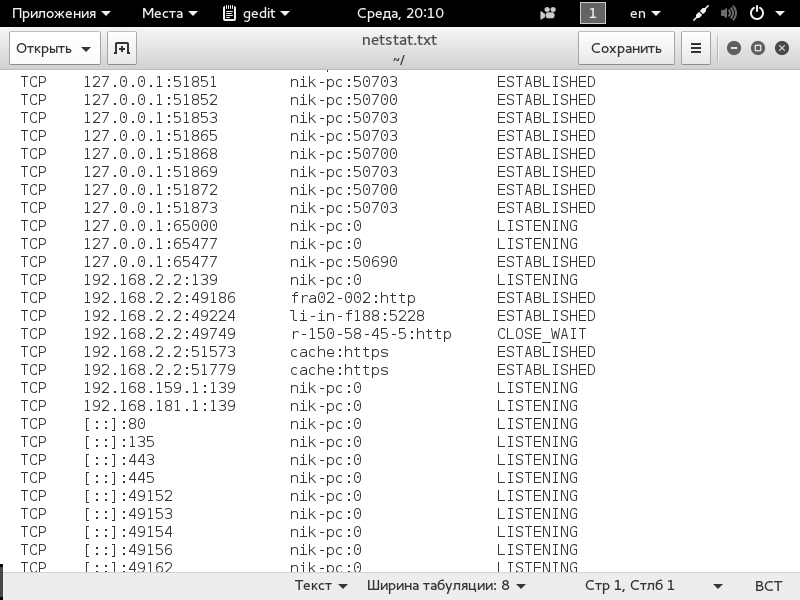
\includegraphics[width=0.6\textwidth]{images/18.png}
	\caption{Расшифровка}
\end{figure}

\newpage
\subsection{Использование GPG с помощью консольного интерфейса}
Эксперименты будут проводиться на другой машине.

\begin{verbatim}  
# gpg2 --gen-key
gpg (GnuPG) 2.0.28; Copyright (C) 2015 Free Software Foundation, Inc.
This is free software: you are free to change and redistribute it.
There is NO WARRANTY, to the extent permitted by law.

Выберите тип ключа:
   (1) RSA и RSA (по умолчанию)
   (2) DSA и Elgamal
   (3) DSA (только для подписи)
   (4) RSA (только для подписи)
Ваш выбор? 1
длина ключей RSA может быть от 1024 до 4096 бит.
Какой размер ключа Вам необходим? (2048) 2048
Запрошенный размер ключа - 2048 бит
Выберите срок действия ключа.
         0 = без ограничения срока действия
      <n>  = срок действия ключа - n дней
      <n>w = срок действия ключа - n недель
      <n>m = срок действия ключа - n месяцев
      <n>y = срок действия ключа - n лет
Срок действия ключа? (0) 
Срок действия ключа не ограничен
Все верно? (y/N) y

GnuPG необходимо составить ID пользователя в качестве идентификатора ключа.

Ваше настоящее имя: console_key
Адрес электронной почты: console_key@mail.com
Комментарий: 
Вы выбрали следующий ID пользователя:
    "console_key <console_key@mail.com>"

Сменить (N)Имя, (C)Комментарий, (E)Адрес или (O)Принять/(Q)Выход? O
Для защиты закрытого ключа необходима фраза-пароль.

Необходимо получить много случайных чисел. Желательно, чтобы Вы
в процессе генерации выполняли какие-то другие действия (печать
на клавиатуре, движения мыши, обращения к дискам); это даст генератору
случайных чисел больше возможностей получить достаточное количество энтропии.
Необходимо получить много случайных чисел. Желательно, чтобы Вы
в процессе генерации выполняли какие-то другие действия (печать
на клавиатуре, движения мыши, обращения к дискам); это даст генератору
случайных чисел больше возможностей получить достаточное количество энтропии.


gpg: ключ 89F19600 помечен как абсолютно доверенный.
открытый и закрытый ключи созданы и подписаны.

gpg: проверка таблицы доверия
gpg: требуется 3 с ограниченным доверием, 1 с полным, модель доверия PGP
gpg: глубина: 0  верных:   2  подписанных:   0  доверие: 0-, 0q, 0n, 0m, 0f, 2u
pub   2048R/89F19600 2016-09-01
      Отпечаток ключа = C41D 74C4 5885 47F3 117B  D7AC 8197 07B1 89F1 9600
uid     [абсолютное] console_key <console_key@mail.com>
sub   2048R/4E4FB84D 2016-09-01

root@kali:~# gpg2 --list-keys
/root/.gnupg/pubring.gpg
------------------------
pub   2048R/27FB9D6C 2016-08-31
uid     [абсолютное] kali-linux <kali-linux@mail.com>
sub   2048R/FE5B0496 2016-08-31

pub   2048R/DDCCD31E 2016-08-31
uid     [неизвестно] windows <windows@mail.com>
sub   2048R/728F8FE0 2016-08-31

pub   2048R/89F19600 2016-09-01
uid     [абсолютное] console_key <console_key@mail.com>
sub   2048R/4E4FB84D 2016-09-01


root@kali:~# gpg2 --export --armor 89F19600
-----BEGIN PGP PUBLIC KEY BLOCK-----
Version: GnuPG v2

mQENBFfIcKcBCADpMfRp40BhT2quJ2e+RtL+TdMFW0mSDuQsci6BW7Hp5wMBjlCm
ae+OsgGFsC3vRj3K+YmE2ZYefG4DKa7XKbw5+xifDqRYyMFt7RUNoGpa+kNWjkZu
/JHTZLZ5bQdHFVE01y+z+01pEKioAcV8YFpHKZViKExmjRXhYAEcRo9Eg1ZzkKXn
XWOVK036blP2sVGlSyQnscE9zwYCnB7CbQ5geBvH+wjPBnZ+pkuM/kjJbH5q6Pug
djRy5ihu5ZO3rwrV6MPrQSyeDRvd3ovtTc9mMuxrTdGx6BvX3eQ+xiMH4Ecgr7Ys
0x03Swn9zASfx0xOkjhkAOGgKIkrmdyYtlk3ABEBAAG0ImNvbnNvbGVfa2V5IDxj
b25zb2xlX2tleUBtYWlsLmNvbT6JATkEEwEIACMFAlfIcKcCGwMHCwkIBwMCAQYV
CAIJCgsEFgIDAQIeAQIXgAAKCRCBlwexifGWALYDCACJIb1Sq5voeTjJcRRItwZt
JffksLUP7+BN4EvlBbCDHJ022I8Dri+YqnS3fT/K9uKCj4K/podRx3Tl37lpNuUL
v7Jw4mPfFhxPdKsUWrnsx71pXfAymA5rx3BqJBT7hKtNY65B+aXfXNXd94pFMHR5
9RzQ2PMFxXlveGY95vAVy5nXjDy0/38k+DA/Uch/O4YLQ2IkuTyiUt3304MWpSgj
Hhf49E5SVTjIc1X0B+OE1Jv8mfW+v3AaBV7zoSOXYmvKAQ2GcPC6+om1AL4tqVov
n5Zgi3dxnEbD5234EU2DUP6wiK39DcVCKSCYnUJ2vv1mAOWvX2oYTYZklyLMGLyR
uQENBFfIcKcBCADMp9ZxeB0n2jvVKEWVDUvto26w6D9vlzpfyRBGgYqG9/oX26QD
lTkGhXWbk3zpZUPNg2mT/7Fu7KyExPLpRz9hSfy4ExyHH+jab4xZojs4gJ6FhFVS
mb7fuX+xVR1FDrFqTJYj93I+Jx8fVFDLBE8b1exJfvBYozFtxeDeESHh3fjYq9Ul
u77cjyM+lNIS2eooX1YYbwQBhFql6xJPkXDRcGbzVvekxzDngs6Gw6lWNuX43vUX
DwM1vpWY9aMUhUDri2NeaGsD3z4DI7bEK/LtuZTGNwipytHj3UkOlvQD2Vl3Orb3
qLENYuOYqFRXIb5QbmzKejR57uVnko47O+wNABEBAAGJAR8EGAEIAAkFAlfIcKcC
GwwACgkQgZcHsYnxlgBK+gf+KjzSlE8VbIB0IkubAFbObBDYWs9AdfqYX3CEo2LT
wyD6tTVSW5DUY538b/6Y8freMCR8n8oO4yfgRAvbgxnL2+dT2LRACcWPeBmTR2uE
mA9w3LzheAGe8xN5iL+T9UAk+vsM8kex5+3tAO8SlyMgXefYliBqaFWPbYKfaI0M
Pdrx4678ahXNbY02ZkcVjLblvuMoD8FNWvribq6Cv+mhlHlK/i694oQ7l11V/a2k
pc5sFPF1Uo243dhuVPY2nbwYzphVRN/RNDms1+TNa9QLfee2h0jiVaOtVMfQeYlW
FVnf7Ra5XWI833CIDtW2LZhIzlavM1E5ntub47EEnkqYvA==
=NQiy
-----END PGP PUBLIC KEY BLOCK-----
root@kali:~# gpg2 --list-keys
/root/.gnupg/pubring.gpg
------------------------
pub   2048R/27FB9D6C 2016-08-31
uid     [абсолютное] kali-linux <kali-linux@mail.com>
sub   2048R/FE5B0496 2016-08-31

pub   2048R/DDCCD31E 2016-08-31
uid     [неизвестно] windows <windows@mail.com>
sub   2048R/728F8FE0 2016-08-31

pub   2048R/89F19600 2016-09-01
uid     [абсолютное] console_key <console_key@mail.com>
sub   2048R/4E4FB84D 2016-09-01

root@kali:~# gpg2 --armor --encrypt msg.txt
Не задан ID пользователя (можно использовать "-r").

Текущие получатели:

Введите ID пользователя. Пустая строка для завершения: DDCCDD31E
Нет такого ID пользователя.

Текущие получатели:

Введите ID пользователя. Пустая строка для завершения: DDCCD31E
gpg: 728F8FE0: Нет свидетельств того, что данный ключ принадлежит названному пользователю

pub  2048R/728F8FE0 2016-08-31 windows <windows@mail.com>
 Отпечаток главного ключа: BEC1 28EA 73AD A2DB 55FB  1D72 4912 5B62 DDCC D31E
       Отпечаток подключа: 9E6A 202B 8027 A613 92AB  EC22 2602 DB27 728F 8FE0

Нет уверенности в том, что ключ принадлежит человеку, указанному
в ID пользователя ключа. Если Вы ТОЧНО знаете, что делаете,
можете ответить на следующий вопрос утвердительно.

Все равно использовать данный ключ? (y/N) y

Текущие получатели:
2048R/728F8FE0 2016-08-31 "windows <windows@mail.com>"

\end{verbatim}
%\end{document}
